\chapter{General Configuration Management in MADTrack}\label{cap:Milestone3}

One of the main milestones presented within the previous chapter is milestone 3 (codename \emph{G}), which is focused on the development of features related to General
Configuration Management. The main purpose of developing this features as a separate module is to provide an extensible basis for possible future developments of features
unrelated to versioning datasets and models, and more related to basic configuration management mechanisms. In this chapter, a brief introduction to what needs to be developed
will be made, as well as an analysis of the requirements that will need to be developed for this milestone, which will result into a diagnosis of the most suitable architecture
and application type for this module.

\section{Introduction}

The partial objectives of the project are related to configuration management applied to datasets and models, but the development of such a system will depend on more generic
configuration management mechanisms. In fact, it is shown on the project's roadmap (\emph{figure \ref{fig:roadmap}}) that the development of the general configuration management
features is crucial for initiating the development in the rest of the modules. Hence, the development of this module will be focused on creating mechanisms that interact
synergically with the rest of the modules, mainly in the cases where commits to remote or local repositories are required.

\section{Requirements analysis for milestone 3}

The main purpose of analysis is to define the most suitable way to proceed with the development of the prototypes. In this case, the functionalities provided by Git are the 
are the ones more suitable to use in the context of development. This Prototype interacts with all those prototypes that require to integrate changes to the system, such as 
tracking and committing changes within a dataset or a model.

\subsection{Requirements involved}

The requirements involved within this milestone have already been listed within \emph{table \ref{tab:requirementsMilestone3}}. These requirements all belong to prototype \emph{G1}, which
is the first one to be completed, and the only one belonging to this milestone.

Additionally, prototypes within milestone 3 require the satisfaction of the non-functional requirements listed within \emph{table \ref{tab:nonFunctionalRequirements}}.

\subsection{Integration with the rest of the system}

Prototype G1 is the prototype which constitutes the core dependency for the most prototypes to be developed within the other two milestones. The depending prototypes are D2, which
needs a mechanism for committing changes made to DVC's files, and M2, which would potentially need a mechanism for committing metadata stored about training configurations.

\begin{figure}[H]
    \centering
    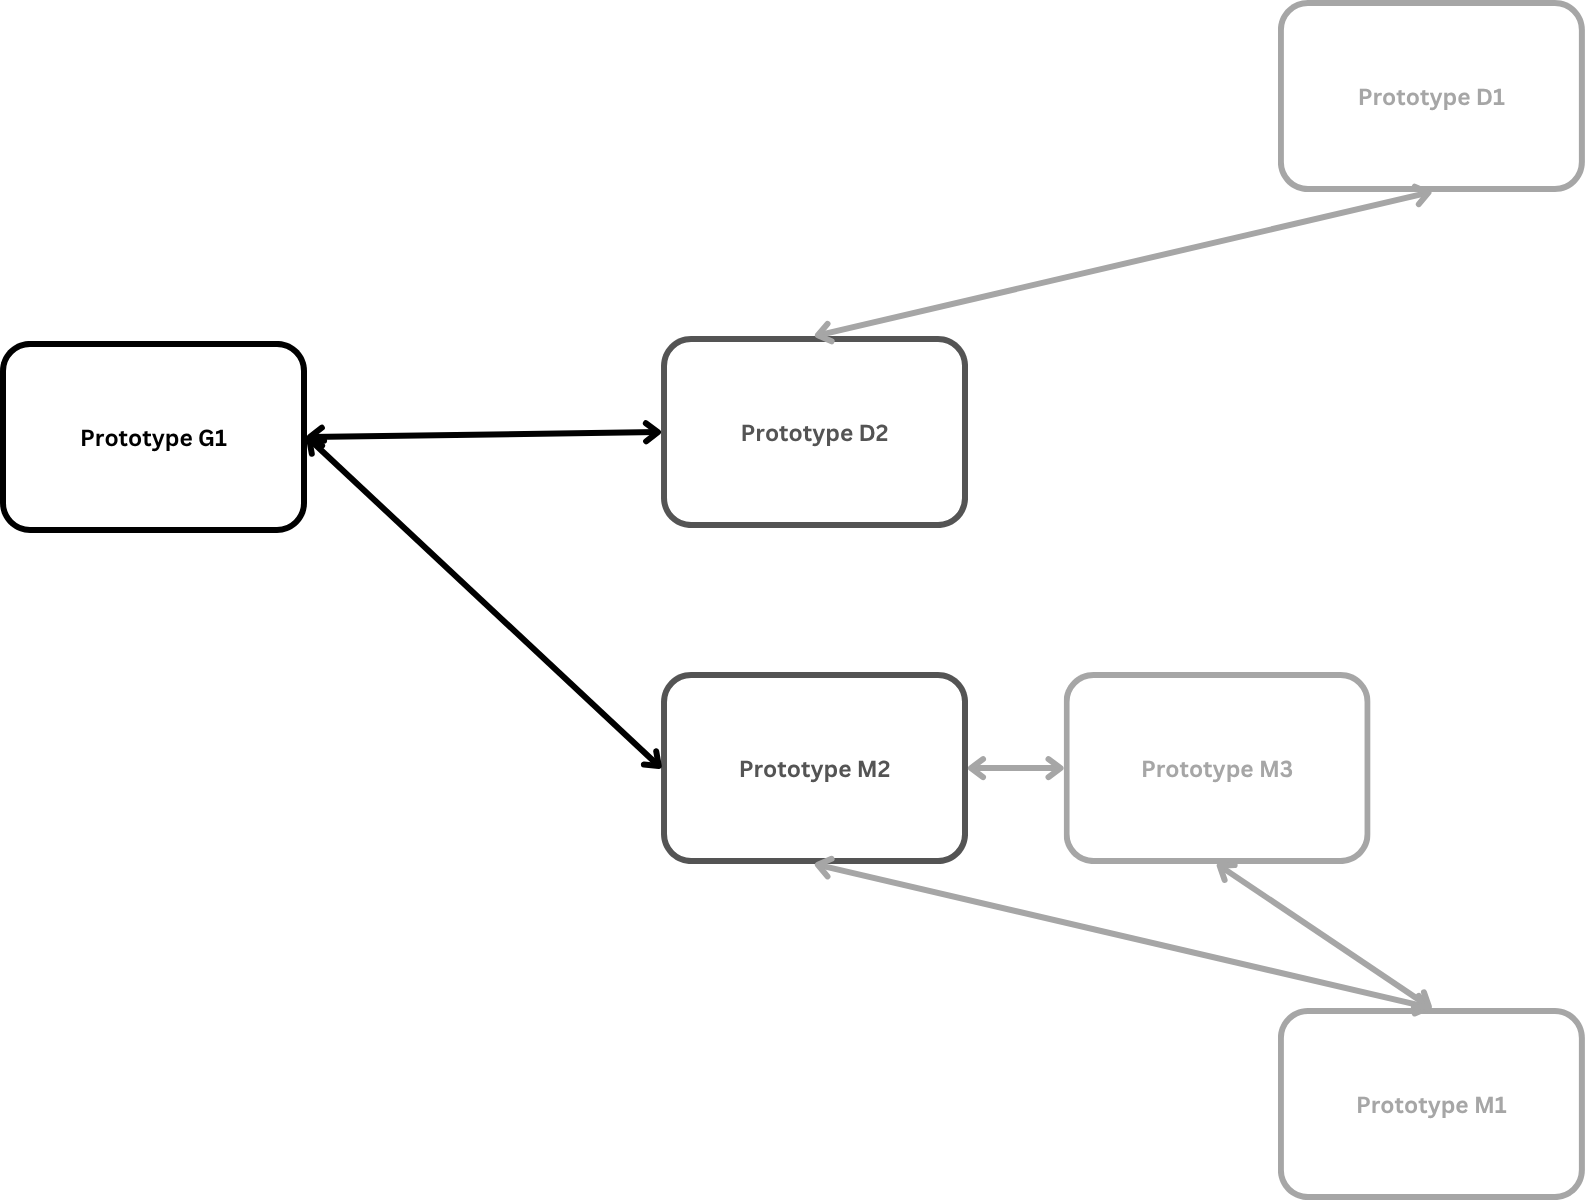
\includegraphics[width=0.7\textwidth]{figs/G-dependencies.png}
    \caption{Dependencies between prototypes of milestone 3 and the rest of the target system, shown by an interaction diagram.}
\end{figure}

\subsection{Architecture analysis}

The nature of the requirements of the milestone describe that multiple aspects shall be handled: The user may want to push their changes to either a local or remote repository. 
And the way to commit changes differs from whether the committed item is a dataset (The information of the DVC tracking file must be committed) or an \acrshort{AI} model (whole model folders can be committed from a repository within
the remote tracking server). Additionally, as versions would be defined by the commit name, a functionality to retrieve the name of the active commit could be useful.

Considering these needs and the aforementioned requirements, the conclusion reached was that the most suitable architecture for the modules of milestone 3 would mainly consist of
a monolithic application, with the possibility for it to connect momentarily to a remote repository server to push changes.

\subsection{Application type analysis}

Due to the reasons described in the previous subsection, the best option for the development of prototypes of this milestone shall be a wrapper library that encapsulates Git
operations. A library that allows to commit to local or remote repository independently on the item to be committed, facilitating thus its integration with toolkits that enable the 
tracking of datasets and models.

\subsection{Toolkit analysis}

Any API or library handling basic Git committing operations will be helpful for the development of the prototypes. Details on the final toolkit used are described in the coming subsections.

\section{Prototype design and development}

Within the coming sections, details for the design, implementation and testing phases of the development of this milestone's prototypes are shown in a sequential order. Since this milestone
is composed of a single prototype, its development will be described in the following subsection.

\subsection{Prototype \emph{G1}}

Prototype G1 is the only prototype of milestone 3, and the core dependency of many other prototypes. It has the aim of bringing basic Git operations to a library accessible to the end users.

\subsubsection{Design for prototype \emph{G1}}

The use case diagram for prototype \emph{G1} is shown in \emph{figure \ref{fig:useCaseG1}}.

\begin{figure}[H]
    \centering
    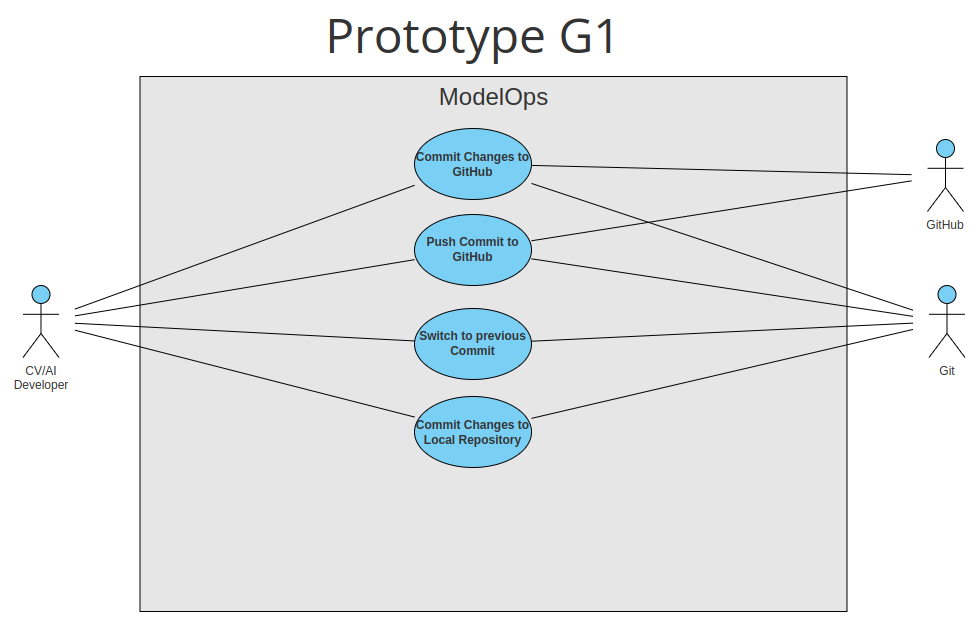
\includegraphics[width=0.7\textwidth]{figs/use-case-G1.png}
    \caption{Use case diagram for prototype \emph{G1}.}
    \label{fig:useCaseG1}
\end{figure}

Taking a look at this diagram, it is clear that there is a crucial component needed to carry out this prototype: a component that handles the Git \emph{commit} and \emph{push} operations, along with
the possible exceptions that this may generate.

\paragraph{Prototype \emph{G1} components}

\begin{itemize}
    \item \textbf{Commit Manager: }a component that will contain the functions for managing both local and remote repositories, as well as operations for chaning the active commit (\emph{checkout}).
    
    \item \textbf{Commit Exceptions: }A package that includes some special exceptions that can be raised by the Commit Manager.
\end{itemize}

\paragraph{Prototype \emph{G1} components' contents}\mbox{}\\

This paragraph will address the question of which information is stored by each of the classes and what functions will be contained within them. The methods of each component 
are described within the following lists.

\subparagraph{Commit Manager}\mbox{}\\


The attributes of this component are:

\begin{itemize}
    \item \texttt{repo\_path}: a character string that contains the path to the repository where the commits will be stored.
\end{itemize}

The methods of this component are:

\begin{itemize}
    \item \texttt{commitLocal}: processes changes over a repository to create a new version of it.
    \item \texttt{commitRemote}: processes changes over a repository to create a new version of it and push it to a remote repository.
    \item \texttt{checkoutCommit}: changes the pointer of the repository to a specific commit. The effect of this method is that the changes made to a file are temporarily 
    reverted to a previously defined state of the files within the repository. 
    \item \texttt{findCommits}: Finds the commits within a repository that have a certain name, and stores them into a map object with the dates of the commits and their UID.
    This is thought to be used for searching multiple commits within the same name in order to select to which one the user will switch to.Added in later development stages of the project due to a need encountered during the development of milestone 2.
    \item \texttt{getCurrentCommitName}: returns the active commit's name. As well as the previous method, it was developed on a later development stage to satisfy a need encountered in other milestone.
\end{itemize}

\paragraph{Prototype \emph{G1} Class Relationships}

\begin{itemize}
    \item Dependency - Commit Manager $\rightarrow$ Commit Exceptions
    \item Dependency - Commit Manager $\rightarrow$ GitPython
\end{itemize}

\paragraph{Design output}\mbox{}\\

The output design class diagram for prototype \emph{G1} is shown in \emph{figure \ref{fig:G1classDiagram}}.

\subsubsection{Implementation for prototype \emph{G1}}

This section addresses questions about the programming language used, the libraries imported and a high-level description of the implementation of the components' methods.

\paragraph{Programming language} \mbox{}\\

Given the notorious availability of tools, frameworks and libraries in the language, as well as the balance between the efectiveness easiness of use the selected language for the development
of this prototype is Python.

\paragraph{Libraries used} \mbox{}\\

The libraries used for the implementation of this prototype are:

\begin{itemize}

    \item \textbf{\emph{GitPython}: }the selected toolkit to handle \emph{commit}, \emph{push} and \emph{checkout} operations.
    \item \textbf{\emph{Logging}: }A library that enables the creation of log files and manages log operations within any Python application.
    \item \textbf{\emph{OS}: }enables interactions with the operating system, mainly used in this prototype for verifying the existence of particular files and directories.

\end{itemize}

\paragraph{Commit Manager method flows} \mbox{}\\

\textbf{Commit Manager - Constructor}
\begin{enumerate}
    \item When the function is called, the code validates the existence of a local repository on the specified path.
    \item If the repository is not found, an existing exception for non-existing repositories is raised.
    \item If the repository is found, the attribute \texttt{repo\_path} is set to the path of the repository.
    \item The function returns the instance of the class.
\end{enumerate}

\textbf{Commit Manager - commitLocal}

\begin{enumerate}
    \item Upon being called, the function checks whether the repository is dirty (there are any uncommitted changes).
    \begin{enumerate}
        \item If the repository is not dirty (nothing is to be committed), an error for such situation is raised.
    \end{enumerate}

    \item If there are uncommitted changes, the function iterates over the list of files to be added for the commit.
    \begin{enumerate}
        \item If the file is not present within the repository or is present as a directory, a warning will be left on the logs as part of the handling routine of an exception
        for such a situation.

        \item If the file is present within the repository, but it has not any uncommitted changes, it is removed from the list of files to be added for the commit as part of 
        handling an exception created for such a situation.
    \end{enumerate}

    \item Once all files have been checked, the function checks the validity of the provided commit message.
    \begin{enumerate}
        \item A commit message will be valid if it complies within the string validity standards: does not exceed length limitations, and the format passes a security check (it does not contain potential code injection substrings).
        \item If a commit message is not valid, an error for such situation is raised.
    \end{enumerate}

    \item If the commit message is valid, the function adds the files to the commit list.
    
    \item Finally, the function commits the changes to the repository.
    \begin{enumerate}
        \item Should the commit transaction fail, the error shall be processed for the user to know and then returned in a logging message.
    \end{enumerate}

    \item The function returns the number of files that were committed.
\end{enumerate}

\textbf{Commit Manager - commitRemote}
\begin{enumerate}
    \item Upon being called, the function executes the \texttt{commitLocal} method.
    \item Provided the success of the previous method call, the function pushes the changes to a remote repository.
    \begin{enumerate}
        \item Should the commit transaction fail, the error shall be processed for the user to know and then returned in a logging message.
    \end{enumerate}
    \item The function returns the number of files that were committed.
\end{enumerate}

\textbf{Commit Manager - checkoutCommit}
\begin{enumerate}
    \item Upon being called, the function checks whether the repository is dirty (there are any uncommitted changes).
    \begin{enumerate}
        \item If the repository is dirty (something is to be committed), an error for such situation is raised.
    \end{enumerate}

    \item the function checks whether the provided commit ID is valid (according to the string validity standards).
    \begin{enumerate}
        \item If the commit ID is not valid, an error for such situation is raised.
    \end{enumerate}

    \item Next, the function checks the validity of the instance number (one of the provided parameters). This instance number represents, among many commits with the same name, which one is to be checked out.
    \begin{enumerate}
        \item If the instance number is a negative number, an error for such situation is raised.
    \end{enumerate}

    \item The function checks whether there are commits with the provided name in the repository.
    \begin{enumerate}
        \item If no commits are found, an error for such situation is raised.
    \end{enumerate}

    \item If there are commits with the provided name, the function selects the commit holding the position specified by the instance parameter.
    \begin{enumerate}
        \item If the instance number is higher than the number of commits, the function selects the oldest commit with this name. On the other side, should this parameter not be specified, the latest instance will be selected.
    \end{enumerate}

    \item The function performs the checkout operation to the specified commit.

    \item The function returns the position of the selected commit within the commit list.
\end{enumerate}

\textbf{Commit Manager - findCommits}
\begin{enumerate}
    \item The function uses \emph{GitPython} to instantly retrieve the list of commits in the repository.
\end{enumerate}

\textbf{Commit Manager - getCurrentCommitName}
\begin{enumerate}
    \item The function uses \emph{GitPython} to retrieve the first line of the active commit's message.
\end{enumerate}

\subsubsection{Testing for prototype \emph{G1}}

Within the following sections, details for the testing phase of prototype \emph{G1} are shown. This includes the description of the different equivalence classes found for the prototype, and the
errors found and lessons learned during the verification of the prototype.
\newpage
\paragraph{Equivalence classes for Commit Manager}

\subparagraph{Commit Manager - Constructor} \mbox{}\\
\begin{enumerate}
    \item \texttt{repo\_path} exists, is a directory and contains a local repository.
    \item \texttt{repo\_path} is not a valid Local Repository.
\end{enumerate}

\subparagraph{Commit Manager - commitLocal} \mbox{}\\
\begin{enumerate}
    \item The list of files to commit is not empty and the commit message is valid.
    \item The repository to commit is not dirty.
    \item The list of files to commit is empty.
    \item The commit message is not valid.
    \item After checking file validity, the list of files to commit is empty.
\end{enumerate}

\subparagraph{Commit Manager - checkoutCommit} \mbox{}\\
\begin{enumerate}
    \item All parameters are valid.
    \item The commit ID is not valid.
    \item The list of commits with the requested name is empty.
    \item instance number is greater than the number of found commits.
    \item instance number is negative.
\end{enumerate}

\paragraph{Test suites for Commit Manager}\mbox{}\\

The test suites for this class can be found in \emph{annex reference placeholder}. % Referencia al Anexo con las tablas (porque pueden ser muy grandes y no es plan). Esto no es prioritario, puede esperar

\paragraph{Errors found and lessons learned}\mbox{}\\

The errors encountered during the course of the testing phase of prototype \emph{G1} are shown in \emph{annex reference placeholder}. % De nuevo, esto puede esperar porque va al anexo

